% FungMod software and methods paper: the manuscript.
%
% Build with `make paper-pdf` (latexmk) from the repository root. The tables
% under tables/ and the figures under figures/ are generated from the recorded
% study results by `python scripts/reproduce_paper.py tables`; they are never
% edited by hand, and the test suite fails when they drift from the results.
\documentclass[11pt,a4paper]{article}

\usepackage[utf8]{inputenc}
\IfFileExists{lmodern.sty}{\usepackage[T1]{fontenc}\usepackage{lmodern}}{}
\usepackage[margin=25mm]{geometry}
\usepackage{amsmath}
\usepackage{booktabs}
\usepackage{tabularx}
\usepackage{array}
\usepackage{graphicx}
\usepackage[round,authoryear]{natbib}
\usepackage{url}
\usepackage[hidelinks]{hyperref}
\urlstyle{same}
\bibliographystyle{plainnat}
% Cosmetic packages a minimal TeX installation may lack; the build does not need them.
\IfFileExists{caption.sty}{\usepackage{caption}\captionsetup{font=small,labelfont=bf}}{}
\IfFileExists{microtype.sty}{\usepackage{microtype}}{}

\title{FungMod: provenance-aware virtual experiments with identifiability
  analysis, preregistered model criticism and cross-solver reproduction for
  fungal substrate degradation}
\author{Felix Laga\thanks{ORCID \url{https://orcid.org/0009-0008-8141-8172}.
    Correspondence: see the repository.}\\
  KU Leuven, Leuven, Belgium}
\date{Draft of 6 October 2026}

\begin{document}
\maketitle

\noindent\textbf{Keywords:} fungal physiology; enzyme kinetics; mechanistic
modelling; parameter identifiability; reproducibility; Python.

\begin{quote}\small
\textbf{Draft status (2026-10-06).} Software and methods paper draft
assembled from the recorded studies in the repository. Every number below is
taken from a checksummed result file named in the text; the tables are
generated \LaTeX{} fragments and the figures generated PDF files, both
written by one command from those files. Items marked \emph{pending} are not
yet recorded. Human review of the biological interpretation is outstanding
and is not asserted here. This draft is not a submission.
\end{quote}

\section{Summary}

FungMod is a Python package for mechanistic virtual experiments on fungal
and enzyme-mediated substrate degradation. A registry of organisms,
substrates, enzymes, environments and parameter records with explicit
provenance and maturity labels is composed through case templates into
well-mixed process models; a compiled numerical core integrates them with
build-time unit resolution; calibration, Bayesian sampling with
identifiability classes, and preregistered model criticism run on the same
models; and the models export to SBML, SED-ML, COMBINE and PEtab so that
independent tools can simulate and fit them. The package is organised
around one rule: a simulation may report only what its inputs and their
evidence support. Unknown inputs stay unknown, exploratory assumptions are
labelled, software verification is never presented as empirical validation,
and every scientific study is run under a plan frozen and digested before
the first fit.

This paper describes the design and demonstrates it on one real organism:
the batch cultures of \emph{Trichoderma harzianum} P49P11 on particulate
cellulose published with the Gelain et al.\ deposit \citep{gelain2020}. We
report (i) a retrospective whole-condition holdout benchmark of the
published hydrolysis candidate, (ii) a posterior-sampling study that
classifies which of its nine constants the published duplicate means
identify, (iii) a preregistered comparison of three added mechanisms, none
of which the data support under the frozen rules, and (iv) a cross-solver
reproduction in which COPASI \citep{hoops2006} simulates the exported PEtab
problem \citep{schmiester2021} to within $1.7\times10^{-8}$ of the
observation scale and then finds an objective 1.3 percent below FungMod's
recorded optimum, which FungMod evaluates to the same value. The last result
is an honest finding against our own optimiser's stopping rule, and the
paper reports it as such.

\section{Statement of need}

Models of fungal degradation are usually published as bespoke equation
sets fitted to one dataset, with units, parameter provenance and the error
model left implicit. Reusing such a model for another strain, substrate or
reactor requires re-deriving all three. General systems-biology tools
(COPASI, SBML-based simulators, PEtab-based estimation frameworks) solve the
simulation and estimation problems well but do not carry the biological
bookkeeping that a degradation study needs: which constant came from which
assay under which conditions, which assay units cannot be converted to
molarity without a specific-activity measurement, which output is a measured
pool and which is a closure ledger, and which claim the evidence actually
licenses. FungMod supplies that bookkeeping as code, keeps it attached to
every output, and hands the resulting problem to the general tools through
the community standards rather than replacing them.

\section{Design}

\subsection{Registry, case templates and maturity}

Every biological input is a registry record with a source, a confidence
level, a validity range and notes. Case templates compose records into a
model config for a (fungus, substrate, environment) triple: state roles,
initial-state mappings, product maps with stoichiometric coefficients that
may be bound to parameter records (a biomass yield \texttt{Y} and its
complement \texttt{1 - Y}), and a list of generic process templates. The
first organism case composes six generic processes (enzyme-explicit
Michaelis-Menten consumption with a yield split, three first-order losses
and two producer-proportional, saturably induced activity syntheses) with no
organism-specific code path. Assay activities (filter-paper units and
beta-glucosidase units) are independent base dimensions of the unit
registry: they cannot be converted to mass or molarity, and a conversion
would have to enter as a sourced parameter.

A run carries a mode (\texttt{scientific} or \texttt{exploratory}) and
every record a maturity. The scientific mode refuses inputs below its
maturity floor; the exploratory mode runs them and labels the output. The
result bundle lists mechanisms, assumptions, provenance, limitations and
suggested experiments next to the trajectories.

\subsection{Compiled process core}

Processes declare required and changed states with units and a rate law on
unit-bearing quantities. The compiled core probes the stoichiometric matrix
from each process's contributions, checks linearity in the rate, resolves
every unit conversion once at build time, and integrates
$\mathrm{d}y/\mathrm{d}t = N\,v(t, y)$ on plain floats with SciPy's LSODA
\citep{virtanen2020}. Every shipped process and modifier supplies a numeric
kernel that reproduces the unit-aware arithmetic in the same operation
order; a process without one uses the recorded unit-aware fallback, never
silently. Trajectories and evaluation counts are identical to the
unit-aware path on every packaged configuration, and solves are 6 to 60
times faster, which is what makes posterior sampling and multi-start
holdout studies affordable.

\subsection{Calibration, posterior sampling and identifiability classes}

A configured-condition predictor rebuilds the model config for each
candidate parameter vector, so a yield bound to a fitted parameter reaches
every place the public path puts it. On top of it: multi-start least
squares in log-parameter space with whole-condition holdouts and a
practical-rank diagnostic; an affine-invariant ensemble sampler
\citep{goodman2010} with checkpointing, autocorrelation-based convergence
rules and a shared observation-noise multiplier sampled jointly with the
parameters; identifiability classes derived from the posterior credible
interval against the prior box (\texttt{identified},
\texttt{weakly\_identified}, \texttt{bounded\_above\_only},
\texttt{bounded\_below\_only}, \texttt{prior\_dominated}, with declared
thresholds); local Fisher information at the best sample; and posterior
predictive bands and coverage. The classes are the operational answer to
``what do these data identify'' that profile-likelihood analysis
\citep{raue2009} gives for a single optimum.

\subsection{Frozen plans and the claim boundary}

Each scientific study is specified by a JSON plan with the data digests,
models, bounds, error model, decision rules, outcome vocabulary and
excluded claims. The plan's SHA-256 is pinned by a test; a change requires
a dated amendment inside the file before any affected run, and every result
cites the digest it ran under. The evaluator that could authorise a
publication claim stays false until replicate-level or independent data
exist.

\subsection{Standards and cross-solver reproduction}

Models export to SBML Level 3 Version 2 \citep{hucka2003} with explicit
numeric unit conversions in the kinetic laws, to SED-ML \citep{waltemath2011}
and COMBINE archives \citep{bergmann2014}, and to PEtab
\citep{schmiester2021}. Two representation choices keep the exported model
faithful where SBML has no construct: a product coefficient bound to a
parameter is written as a separate reaction whose kinetic law multiplies
the process rate by the parameter (or its complement), so the dependence
stays live; and assay-activity units are written as named dimensionless
unit definitions listed in the model notes, with no SI equivalent implied.
A reference simulator independent of the production path checks every
export, and a COPASI driver imports the PEtab problem, corrects the column
weights that COPASI's importer stores as $\sigma$ rather than $1/\sigma^2$,
simulates, fits, and re-evaluates every optimum on the PEtab objective from
COPASI's own time courses.

\section{Results on the Gelain 2020 cultures}

All results are retrospective analyses of published duplicate means that
already informed model development. None is blind, independent or a
validation of biology. Sources: the directories \path{gelain_2020_v2},
\path{gelain_2020_bayesian}, \path{gelain_2020_criticism} and
\path{gelain_2020_petab} under \path{data/benchmarks} in the repository,
each with a plan, a README and digested result files.

\subsection{Whole-condition holdouts of the published candidate}

Table~\ref{tab:table_1_joint_holdouts} lists every model, family and
scenario of the joint benchmark with its held-out error and screen verdict,
and Figure~\ref{fig:figure_1_cellulose_holdouts} shows the frozen held-out
predictions of the hydrolysis candidate and of the re-fitted published
equations against the published means on the three cellulose loadings. The
joint benchmark compares seven model and family combinations against 144
published means (biomass, cellulose or glycerol, filter-paper activity and
beta-glucosidase activity) with each condition held out in turn. On the
three cellulose loadings the activity-driven hydrolysis candidate reaches a
mean normalised held-out mean squared error of 0.092 (training-maximum
normalisation) against 0.0062 for the published equations re-fitted with
their own structure; the published structure fails the complexity screen
that the plan declares, the hydrolysis candidate passes it under the
correlated error assumption only. 33 of 33 folds pass the numerical checks;
6 of 132 optimiser starts fail and are reported. No model is promoted to
validated.

% generated by scripts/reproduce_paper.py tables; do not edit
\begin{table}[tbp]
\footnotesize
\setlength{\tabcolsep}{4pt}
\caption{Whole-condition holdouts of the joint Gelain 2020 benchmark (v2)}
\label{tab:table_1_joint_holdouts}
\begin{tabularx}{\textwidth}{l>{\hsize=0.9596\hsize\raggedright\arraybackslash}X>{\hsize=1.0606\hsize\raggedright\arraybackslash}Xl>{\hsize=0.7071\hsize\raggedright\arraybackslash}X>{\hsize=1.4141\hsize\raggedright\arraybackslash}X>{\hsize=0.8586\hsize\raggedright\arraybackslash}X}
\toprule
Family & Model & Scenario & Parameters & Practical rank & Mean normalized held-out MSE & Complexity screen \\
\midrule
glycerol & effective & primary & 4 & 4 & 0.03287 & passed \\
glycerol & published & primary & 5 & 5 & 0.00594 & passed \\
glycerol & retained & primary & 6 & 6 & 0.02925 & passed \\
cellulose & effective & primary & 8 & 8 & 0.1095 & passed \\
cellulose & published & primary & 20 & 19 & 0.006185 & failed \\
cellulose & hydrolysis & primary & 9 & 9 & 0.09183 & failed \\
cellulose & hydrolysis\_\allowbreak{}retained & primary & 11 & 11 & 0.09316 & failed \\
cellulose & effective & correlated\_\allowbreak{}assumption & 8 & 8 & 0.1139 & passed \\
cellulose & published & correlated\_\allowbreak{}assumption & 20 & 18 & 0.007541 & failed \\
cellulose & hydrolysis & correlated\_\allowbreak{}assumption & 9 & 9 & 0.09497 & passed \\
cellulose & hydrolysis\_\allowbreak{}retained & correlated\_\allowbreak{}assumption & 11 & 11 & 0.09763 & passed \\
\bottomrule
\end{tabularx}
\par\medskip
Folds that passed the numerical checks: 33 of 33; optimiser starts that failed: 6 of 132. Validated: False (retrospective comparison on published means).
\end{table}


\begin{figure}[tbp]
  \centering
  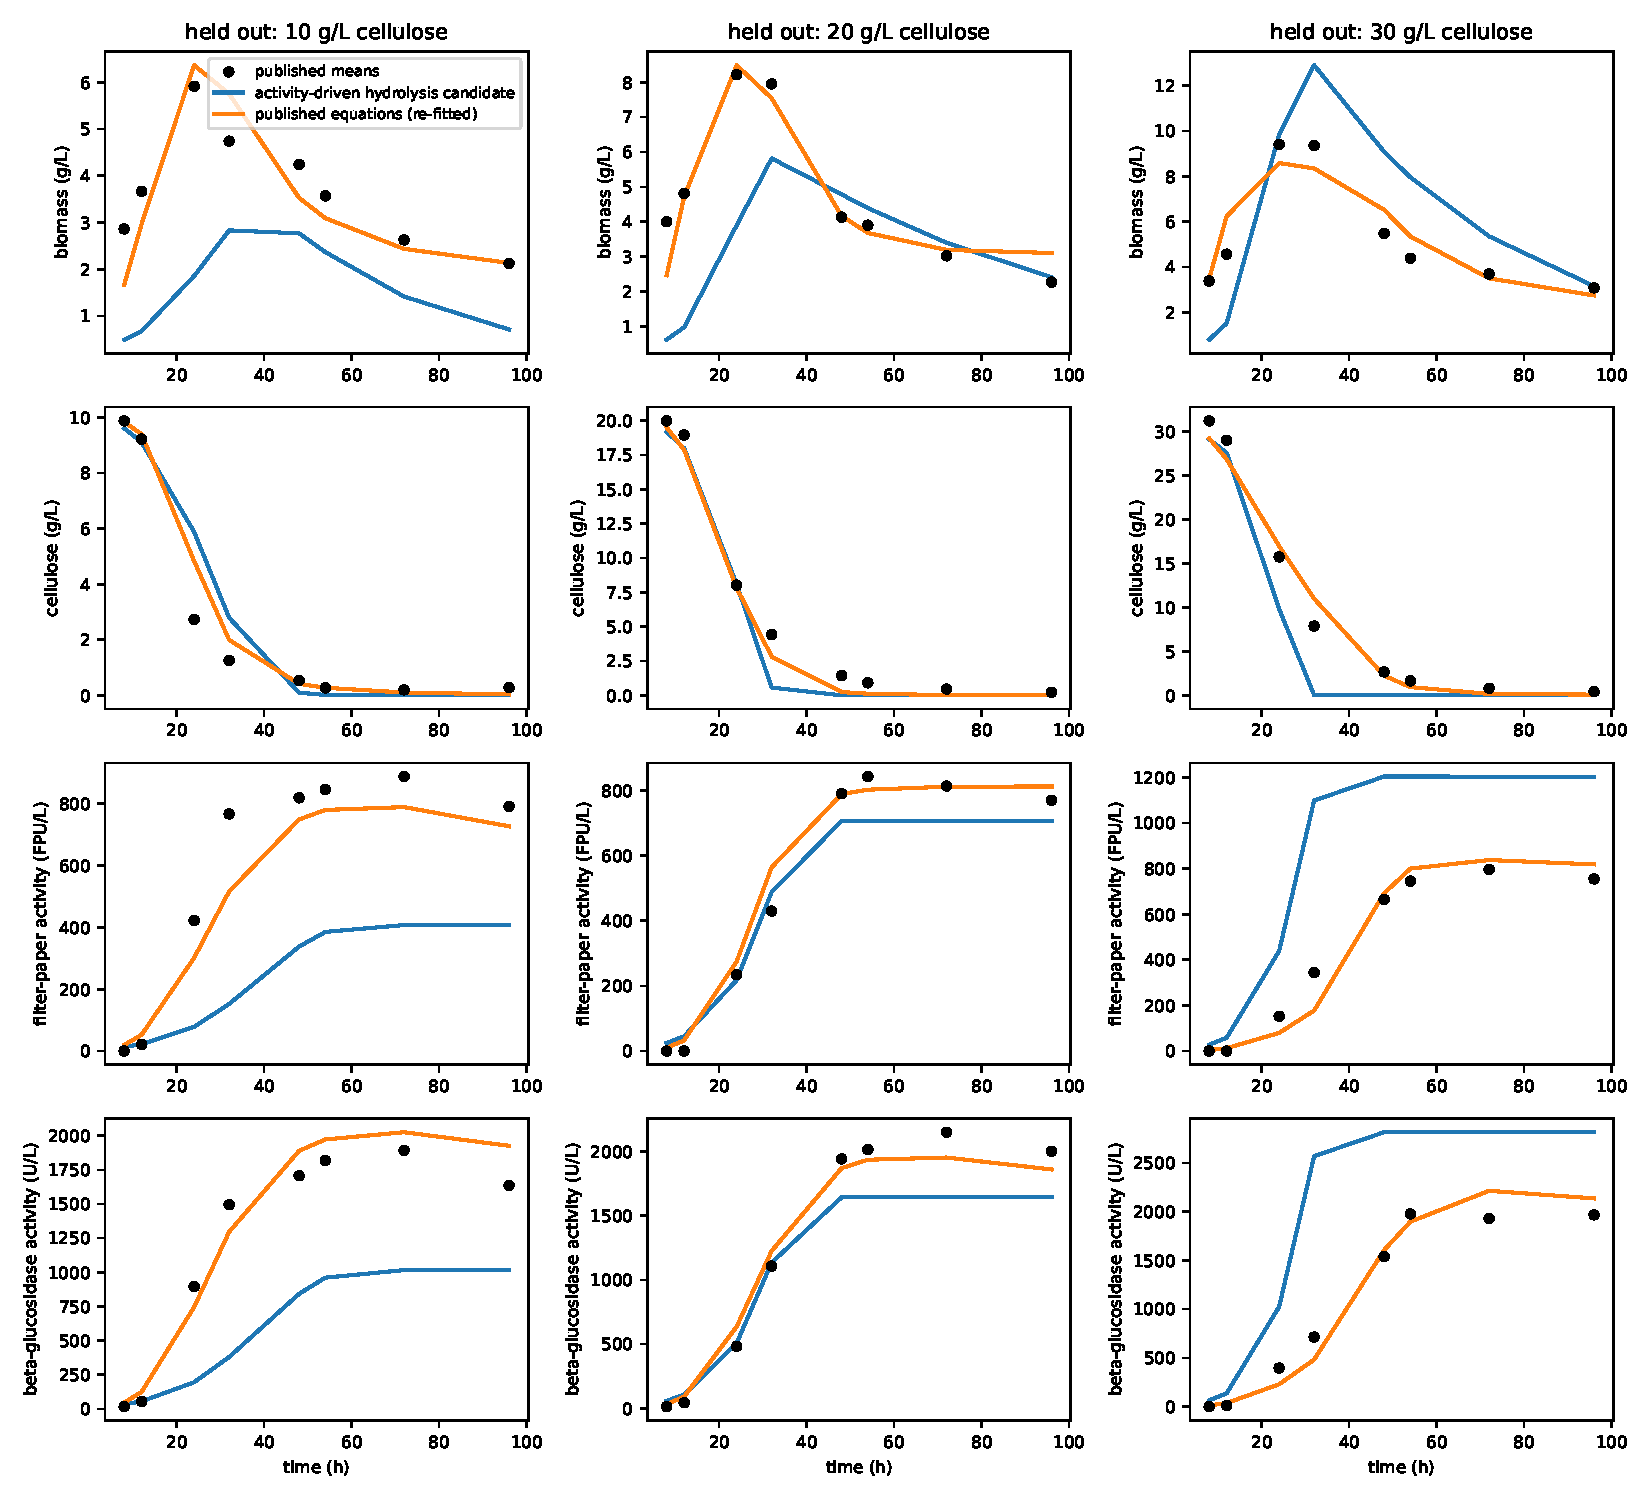
\includegraphics[width=\textwidth]{figures/figure_1_cellulose_holdouts.pdf}
  \caption{Whole-condition holdouts of the joint benchmark on the three
    cellulose loadings. Published means (points) against the frozen held-out
    predictions (lines) of the activity-driven hydrolysis candidate and the
    re-fitted published equations, each loading predicted from a fit to the
    other two (primary scenario). Measurement error is unknown; the points
    are published means.}
  \label{fig:figure_1_cellulose_holdouts}
\end{figure}

\subsection{What the data identify}

Table~\ref{tab:table_2_identifiability} gives the class, posterior median,
credible interval, autocorrelation time and effective sample size of every
constant; Figure~\ref{fig:figure_2_posterior_predictive} shows the
posterior median and the 5 to 95 percent band of the prediction on each
loading, with the published means. Posterior sampling of the nine registry
constants of the hydrolysis candidate (24 walkers, 24\,000 steps, 4\,000
burn-in, log-uniform priors on the declared bounds, one shared noise
multiplier) converges by the declared rule (every autocorrelation estimate
reliable, effective sample sizes 1\,414 to 2\,119, mean acceptance 0.325).
The data identify five constants (the consumption capacity \texttt{k\_h},
the yield \texttt{Y}, the biomass loss rate \texttt{kd} and both specific
production rates \texttt{qF}, \texttt{qB}, with 95 percent credible
intervals of 5 to 16 percent of the prior width in $\log_{10}$), bound the
half-saturation constant \texttt{Kh} from below only, and bound the
induction constant \texttt{K\_ind} and both activity loss rates
\texttt{kF}, \texttt{kB} from above only. The shared noise multiplier's
posterior median is 2.25 (credible interval 1.95 to 2.63) at an assumed 10
percent error, which says that the candidate cannot fit biomass and
cellulose together at that error level. The registry records keep their
frozen point values; the study records which must be read as ranges.

% generated by scripts/reproduce_paper.py tables; do not edit
\begin{table}[tbp]
\footnotesize
\setlength{\tabcolsep}{4pt}
\caption{Identifiability of the nine registry constants of the hydrolysis candidate (BAYES-001)}
\label{tab:table_2_identifiability}
\begin{tabularx}{\textwidth}{l>{\hsize=0.9677\hsize\raggedright\arraybackslash}X>{\hsize=0.8602\hsize\raggedright\arraybackslash}X>{\hsize=0.9677\hsize\raggedright\arraybackslash}X>{\hsize=0.7527\hsize\raggedright\arraybackslash}X>{\hsize=1.4517\hsize\raggedright\arraybackslash}Xll}
\toprule
Constant & Class & Posterior median & 95\% interval & Prior box & Width / prior width (log10) & tau & ESS \\
\midrule
\texttt{k\_\allowbreak{}h} & identified & 0.01848 & [0.00714, 0.0639] & [1e-06, 1] & 0.16 & 305 & 1576 \\
\texttt{Kh} & bounded\_\allowbreak{}below\_\allowbreak{}only & 18.37 & [4.26, 81.9] & [0.001, 100] & 0.26 & 306 & 1567 \\
\texttt{Y} & identified & 0.4783 & [0.328, 0.648] & [0.01, 1] & 0.15 & 299 & 1606 \\
\texttt{kd} & identified & 0.02365 & [0.0114, 0.0392] & [1e-05, 0.5] & 0.11 & 274 & 1754 \\
\texttt{K\_\allowbreak{}ind} & bounded\_\allowbreak{}above\_\allowbreak{}only & 0.0188 & [0.0103, 0.12] & [0.01, 100] & 0.27 & 289 & 1659 \\
\texttt{qF} & identified & 5.606 & [4.2, 7.94] & [0.01, 1e+03] & 0.06 & 324 & 1483 \\
\texttt{kF} & bounded\_\allowbreak{}above\_\allowbreak{}only & 5.331e-05 & [1.21e-06, 0.004] & [1e-06, 0.1] & 0.70 & 278 & 1724 \\
\texttt{qB} & identified & 13.29 & [9.9, 18.7] & [0.01, 3e+03] & 0.05 & 339 & 1414 \\
\texttt{kB} & bounded\_\allowbreak{}above\_\allowbreak{}only & 4.161e-05 & [1.21e-06, 0.0028] & [1e-06, 0.1] & 0.67 & 286 & 1681 \\
\bottomrule
\end{tabularx}
\par\medskip
Shared noise multiplier: median 2.25, 95\% interval [1.95, 2.63] at an assumed 10 percent error. Sampler: 24 walkers, 24000 steps, 4000 burn-in; converged by the declared rule: True; mean acceptance 0.325; effective sample sizes 1414 to 2119.
\end{table}


\begin{figure}[tbp]
  \centering
  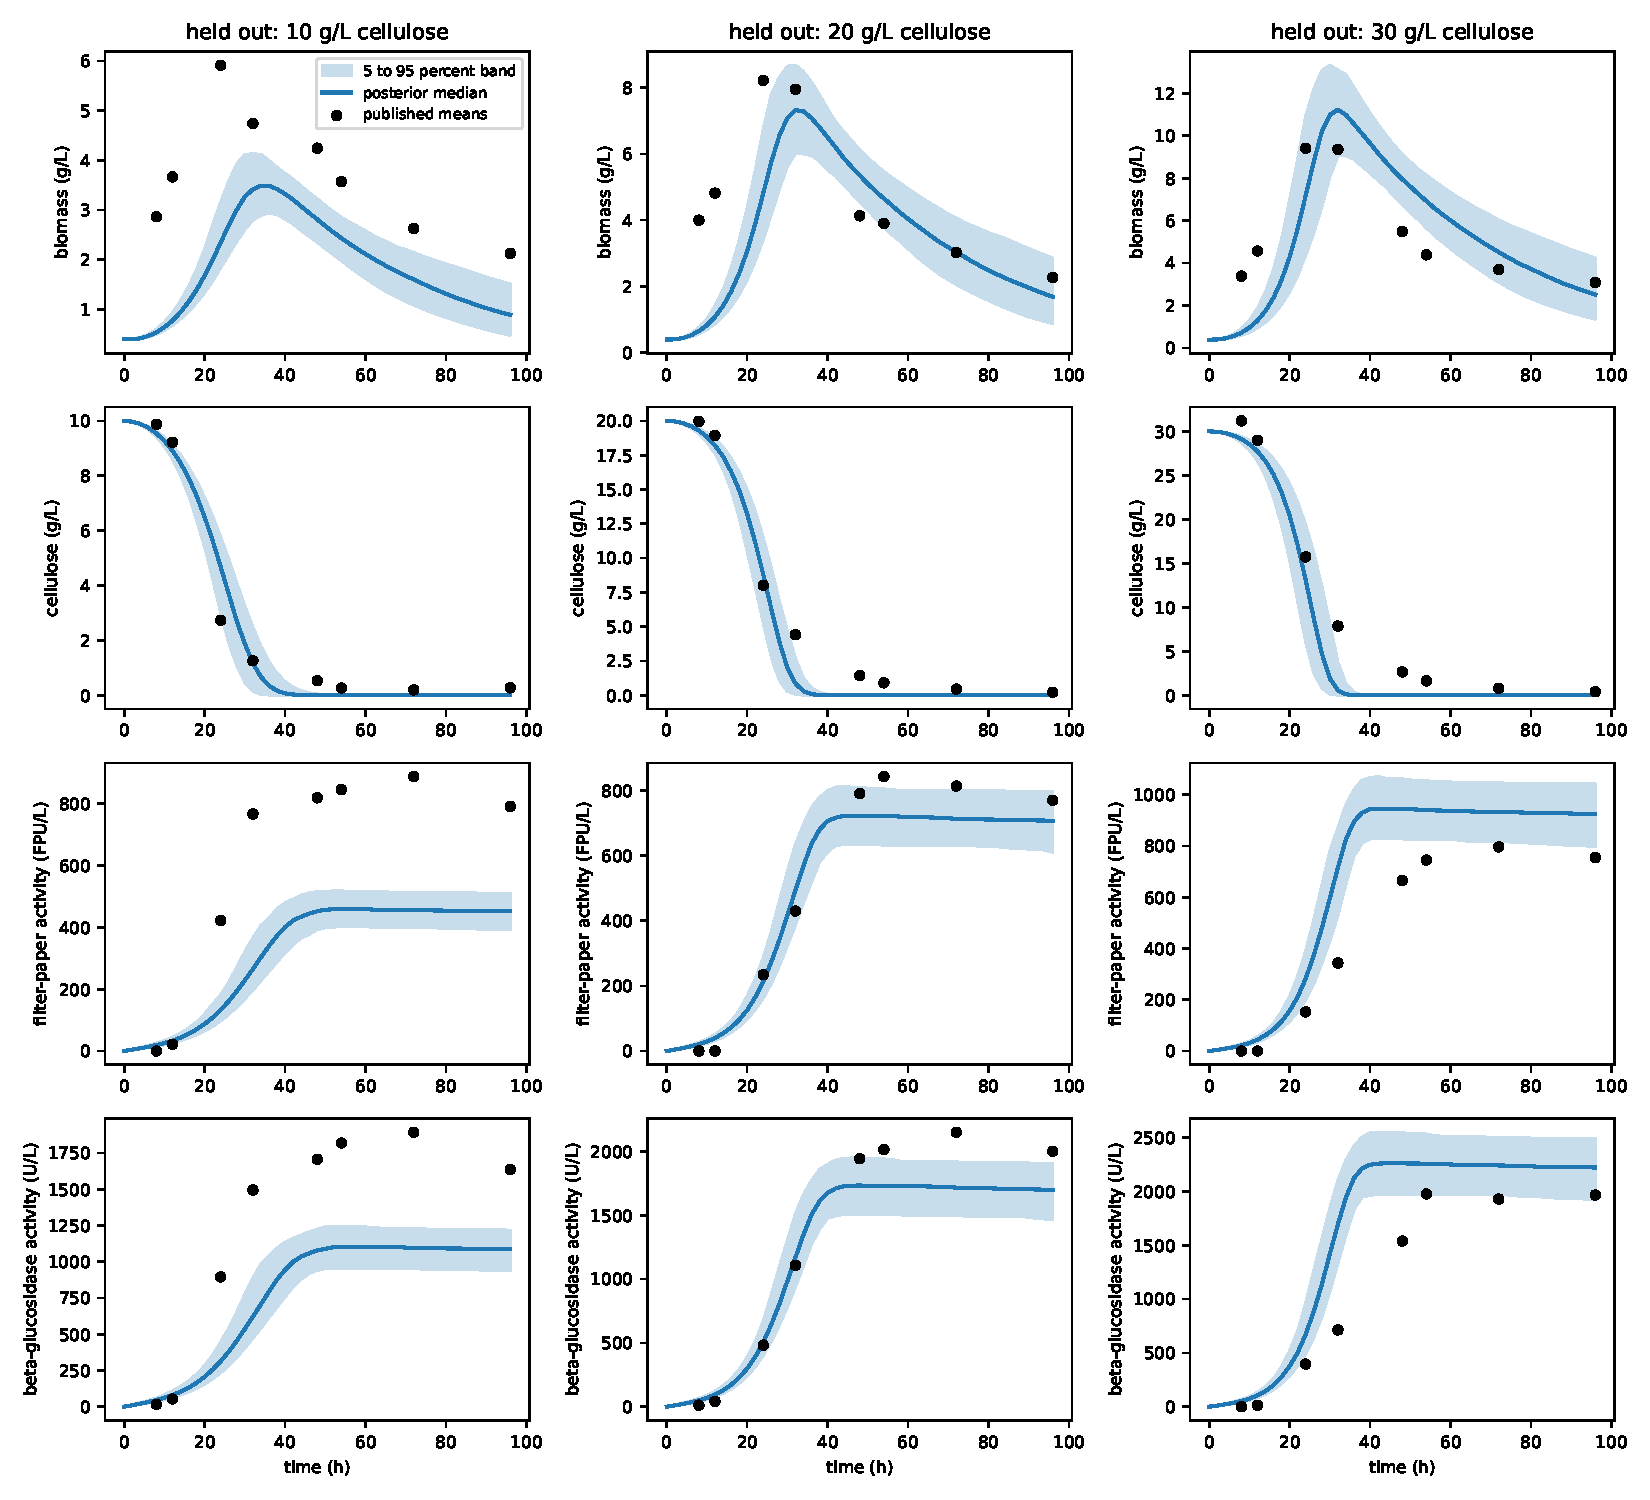
\includegraphics[width=\textwidth]{figures/figure_2_posterior_predictive.pdf}
  \caption{Posterior predictive bands of the hydrolysis candidate on the
    cellulose loadings. Posterior median and the 5 to 95 percent band of
    the model prediction over the posterior samples of the nine registry
    constants (all three loadings fitted; the bands exclude measurement
    noise), with the published means as points.}
  \label{fig:figure_2_posterior_predictive}
\end{figure}

\subsection{Preregistered model criticism}

Tables~\ref{tab:table_3_criticism_stage_a} and
\ref{tab:table_4_criticism_stage_b} carry the holdout screen and the
posterior verdicts per mechanism; Figure~\ref{fig:figure_3_criticism_screen}
shows each mechanism's change in pooled held-out error relative to the
baseline against the screen's thresholds. A frozen plan declared three
mechanisms that could reduce the biomass-cellulose misfit, each added to
the baseline with its bounds, an error model, whole-condition holdouts with
a complexity screen (at least 10 percent pooled held-out improvement, no
observable more than 10 percent worse, full practical rank), decision rules
and an outcome vocabulary. Stage A (least squares, five starts per fold) was
run twice: once with the optimiser as first written, and again under a
dated amendment that declared the finite-difference step after the
cross-solver check below found the first run stopping above the minimum.
The verdicts quoted here are from the second run; the first is kept in the
plan's amendment log and in the ledger. An induction-state memory
(\texttt{M1}) leaves the pooled held-out error unchanged (0.1 percent
better) and makes cellulose three times worse, not supported; a soluble
product pool with Monod uptake and product inhibition (\texttt{M2}) lowers
the pooled held-out error by 23 percent in the primary scenario and 26
percent under the correlated error assumption with every observable better
(biomass by 25 and 36 percent), passing the screen in both;
conversion-dependent accessibility \citep{kadam2004} (\texttt{M3}) does not
improve the pooled error (0.2 percent worse) with its exponent near its
lower bound, not supported. Every fit has full practical rank; every
all-condition fit has at least three of the shared constants on their lower
bounds, and the \texttt{M2} fit puts the initial soluble pool on the top of
its declared range. In the first run \texttt{M2} had failed the screen
because biomass worsened by 31 percent; that was the stalled optimiser, not
the mechanism, and the plan's outcome for \texttt{M2} changed from ``not
supported'' to ``improves fit but unidentified'' when the screen was
recomputed. Stage B sampled one all-condition posterior per addition (24
or 28 walkers, the noise multiplier sampled jointly). \texttt{M1} and
\texttt{M3} ran the planned 8000 steps centred on their first-run fits;
\texttt{M2}, the one addition that passes the screen, was re-run under a
fourth dated amendment from the converged fit with 36000 steps. None of the
three chains met the declared convergence rule, \texttt{M2}'s because its
autocorrelation times grew to 824 to 1393 steps against 28000 post-burn-in
steps, so the plan labels every verdict provisional. Under those labels no
addition restores adequacy: every multiplier interval excludes 1.0, those
of \texttt{M1} and \texttt{M3} overlap the baseline's 2.25 and that of
\texttt{M2} lies below it (1.63 to 2.23, median 1.89). Only the induction
memory constant of \texttt{M1} is weakly identified, while the four
constants of \texttt{M2} are prior dominated or bounded on one side and
the exponent of \texttt{M3} is bounded above only, driven towards the
baseline; posterior predictive coverage with measurement noise is 91 of 96
observations for each. The soluble pool is the one addition the holdouts
support, and the one whose constants the duplicate means do not identify.
The plan's holdout posteriors (amendment 4) sample \texttt{M2} with one cellulose loading held out of the likelihood and score it by held-out posterior predictive coverage at 95 percent with measurement noise: 10 g/L held out, 22 of 32 observations inside; 20 g/L held out, 32 of 32 observations inside; 30 g/L held out, 19 of 32 observations inside. The middle loading is interpolated inside the band; the outer loadings are extrapolated poorly, mainly in the enzyme activities (and in biomass at 30 g/L), and none of the three chains meets the convergence rule, so these are provisional like the rest of stage B.

% generated by scripts/reproduce_paper.py tables; do not edit
\begin{table}[tbp]
\footnotesize
\setlength{\tabcolsep}{4pt}
\caption{Stage A of the preregistered model-criticism study: whole-condition holdouts and the R1 screen}
\label{tab:table_3_criticism_stage_a}
\begin{tabularx}{\textwidth}{>{\hsize=1.3214\hsize\raggedright\arraybackslash}X>{\hsize=0.7500\hsize\raggedright\arraybackslash}X>{\hsize=1.0000\hsize\raggedright\arraybackslash}X>{\hsize=0.5000\hsize\raggedright\arraybackslash}X>{\hsize=0.7143\hsize\raggedright\arraybackslash}X>{\hsize=1.7143\hsize\raggedright\arraybackslash}X}
\toprule
Model & Scenario & Mean normalized held-out MSE & Change vs M0 & Full rank everywhere & Screen (R1) \\
\midrule
M0\_\allowbreak{}baseline & primary & 0.09184 &  & True & passed \\
M0\_\allowbreak{}baseline & correlated\_\allowbreak{}assumption & 0.09324 &  & True & passed \\
M1\_\allowbreak{}induction\_\allowbreak{}state & primary & 0.09173 & +0.1\% & True & failed: pooled normalized held-out error improves by less than the required fraction; an observable worsens by more than the allowed fraction \\
M1\_\allowbreak{}induction\_\allowbreak{}state & correlated\_\allowbreak{}assumption & 0.09606 & -3.0\% & True & failed: pooled normalized held-out error improves by less than the required fraction; an observable worsens by more than the allowed fraction \\
M2\_\allowbreak{}soluble\_\allowbreak{}product\_\allowbreak{}pool & primary & 0.0703 & +23.4\% & True & passed \\
M2\_\allowbreak{}soluble\_\allowbreak{}product\_\allowbreak{}pool & correlated\_\allowbreak{}assumption & 0.0689 & +26.1\% & True & passed \\
M3\_\allowbreak{}conversion\_\allowbreak{}dependent\_\allowbreak{}accessibility & primary & 0.09201 & -0.2\% & True & failed: pooled normalized held-out error improves by less than the required fraction \\
M3\_\allowbreak{}conversion\_\allowbreak{}dependent\_\allowbreak{}accessibility & correlated\_\allowbreak{}assumption & 0.0979 & -5.0\% & True & failed: pooled normalized held-out error improves by less than the required fraction; an observable worsens by more than the allowed fraction \\
\bottomrule
\end{tabularx}
\par\medskip
Per-observable pooled normalized held-out MSE, primary scenario:
\par\medskip
\begin{tabularx}{\textwidth}{>{\hsize=1.3875\hsize\raggedright\arraybackslash}Xll>{\hsize=0.6750\hsize\raggedright\arraybackslash}X>{\hsize=0.9375\hsize\raggedright\arraybackslash}X}
\toprule
Model & biomass & substrate & cellulase\_\allowbreak{}activity & beta\_\allowbreak{}glucosidase\_\allowbreak{}activity \\
\midrule
M0\_\allowbreak{}baseline & 0.07863 & 0.01323 & 0.1603 & 0.1152 \\
M1\_\allowbreak{}induction\_\allowbreak{}state & 0.06378 & 0.04101 & 0.1542 & 0.1079 \\
M2\_\allowbreak{}soluble\_\allowbreak{}product\_\allowbreak{}pool & 0.0592 & 0.01128 & 0.127 & 0.08372 \\
M3\_\allowbreak{}conversion\_\allowbreak{}dependent\_\allowbreak{}accessibility & 0.07387 & 0.01209 & 0.1648 & 0.1173 \\
\bottomrule
\end{tabularx}
\end{table}


% generated by scripts/reproduce_paper.py tables; do not edit
\begin{table}[tbp]
\footnotesize
\setlength{\tabcolsep}{4pt}
\caption{Stage B of the model-criticism study: adequacy, identification and coverage per added mechanism}
\label{tab:table_4_criticism_stage_b}
\begin{tabularx}{\textwidth}{>{\hsize=1.0829\hsize\raggedright\arraybackslash}X>{\hsize=0.7024\hsize\raggedright\arraybackslash}Xll>{\hsize=0.6439\hsize\raggedright\arraybackslash}X>{\hsize=1.4049\hsize\raggedright\arraybackslash}X>{\hsize=0.7610\hsize\raggedright\arraybackslash}X>{\hsize=1.4049\hsize\raggedright\arraybackslash}X}
\toprule
Model & Chain & Converged & R1 holdout & R2 multiplier interval & R3 added-parameter classes & Coverage (95\%, with noise) & Outcome \\
\midrule
M1\_\allowbreak{}induction\_\allowbreak{}state & 24 walkers x 8000 steps & False & False & [1.87, 2.53] & \texttt{kz\_\allowbreak{}loss} weakly\_\allowbreak{}identified & 91/96 & not supported (fails R1) (provisional) \\
M2\_\allowbreak{}soluble\_\allowbreak{}product\_\allowbreak{}pool & 28 walkers x 36000 steps & False & True & [1.63, 2.23] & \texttt{mu} bounded\_\allowbreak{}below\_\allowbreak{}only, \texttt{Ks} prior\_\allowbreak{}dominated, \texttt{Ki} prior\_\allowbreak{}dominated, \texttt{P0} bounded\_\allowbreak{}below\_\allowbreak{}only & 91/96 & improves fit but unidentified (R1, not R3) (provisional) \\
M3\_\allowbreak{}conversion\_\allowbreak{}dependent\_\allowbreak{}accessibility & 24 walkers x 8000 steps & False & False & [1.94, 2.62] & \texttt{n} bounded\_\allowbreak{}above\_\allowbreak{}only & 91/96 & not supported (fails R1) (provisional) \\
\bottomrule
\end{tabularx}
\par\medskip
M0 is the baseline: its all-condition posterior is BAYES-001 (Table 2), which R1 and R3 do not address.
\end{table}


\begin{figure}[tbp]
  \centering
  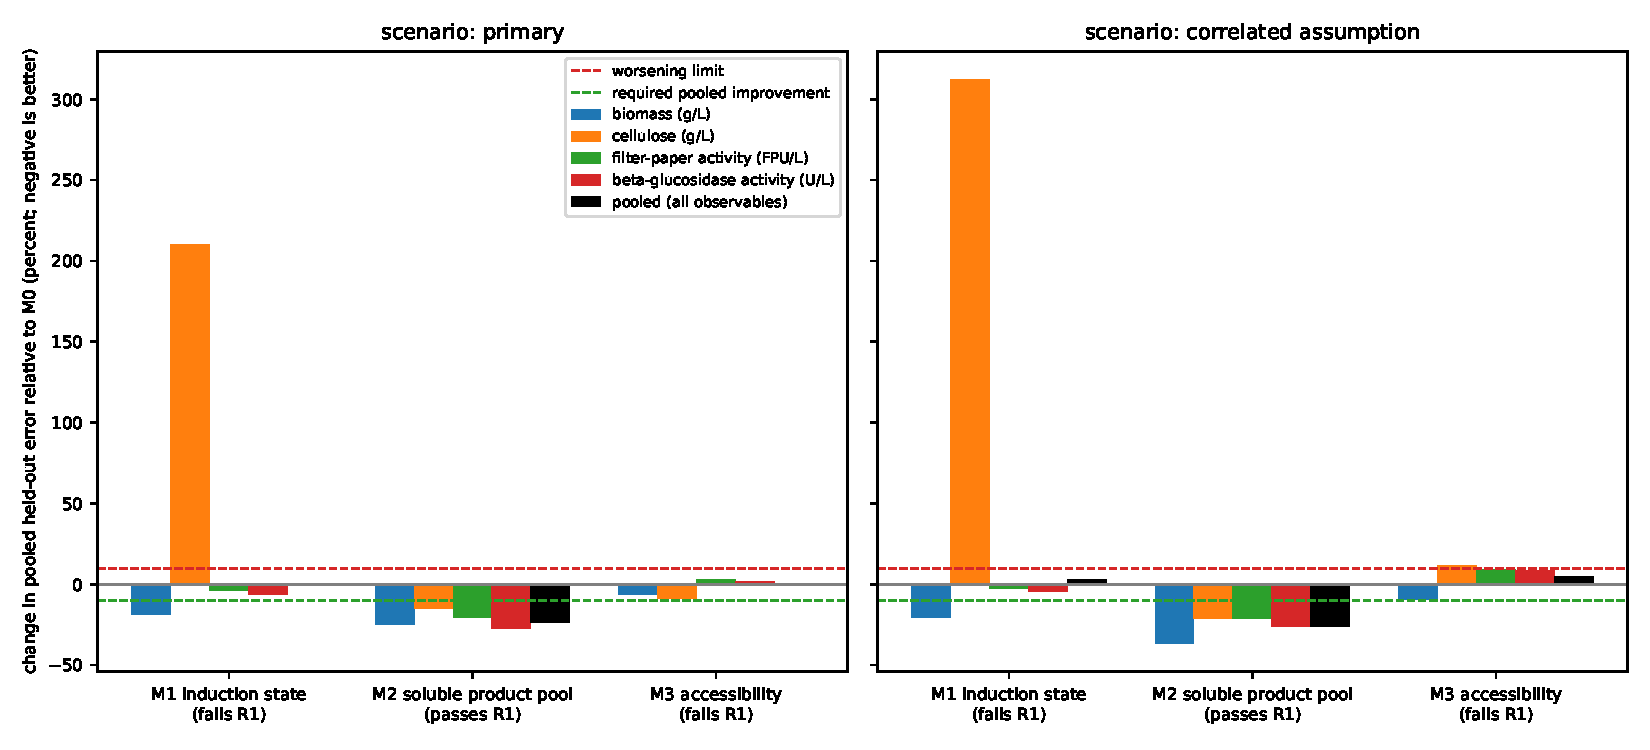
\includegraphics[width=\textwidth]{figures/figure_3_criticism_screen.pdf}
  \caption{Stage A holdout screen of the model-criticism study. Change in
    the pooled held-out normalised error of each candidate mechanism
    relative to the baseline M0, per observable and pooled, in both error
    scenarios; the dashed lines are the plan's screen thresholds (at least
    10 percent pooled improvement, no observable more than 10 percent
    worse).}
  \label{fig:figure_3_criticism_screen}
\end{figure}

\subsection{Cross-solver reproduction}

Table~\ref{tab:table_5_cross_solver} records the gates, the objectives and
the parameter agreement. Figure~\ref{fig:figure_4_cross_solver} plots the
objective at the recorded optimum, after COPASI's local fit and at the end
of its ten random starts. The baseline problem (three loadings, four
observables, 96 measurements, nine parameters on a $\log_{10}$ scale with
the criticism plan's bounds, $\sigma$ equal to each observable's maximum
over the loadings) was exported as a PEtab problem and reproduced in COPASI
4.48 under a frozen plan. The first run found a defect in our own
optimiser. At FungMod's then recorded optimum (objective 4.0307) COPASI's
time courses differed from the compiled core by at most $1.7\times10^{-8}$
of $\sigma$, but COPASI's Levenberg-Marquardt fit from the same point
reached 3.9803 and the best of ten seeded random starts 3.9768, 1.3 percent
lower, and FungMod's compiled core evaluated that point to the same
objective (relative difference $7\times10^{-9}$). The solvers agreed; the
optimisers did not. The cause, recorded in a dated amendment of the
criticism plan, was the finite-difference Jacobian: with scipy's default
step of about $1.5\times10^{-8}$ the differences were dominated by the
adaptive ODE integrator's step noise (derivative norms for the weakly
entering constants fifteen times their converged values), and the trust
region collapsed above the minimum with every start reporting a satisfied
step tolerance. Declaring a log-space difference step of $10^{-3}$, as the
earlier benchmark plan already did, moved every start of the baseline to
the same minimum (objective 3.97607, cost spread across five starts
$5\times10^{-6}$, projected gradient norm $2.5\times10^{-3}$ in log space
against 0.22 before). Stage A of the criticism study was re-run under the
amendment and the cross-solver study was re-run against the new reference:
COPASI's local fit now reaches 3.9760718 against FungMod's 3.9760719
(relative difference $2.5\times10^{-8}$), every parameter agrees to better
than $10^{-4}$ relative, three constants (\texttt{K\_ind}, \texttt{kF},
\texttt{kB}) sit on their lower bounds in both solvers, and no random start
goes lower. Outcome in the plan's vocabulary: \texttt{reproduced}. The
episode is reported in full because it is the kind of defect that a
cross-solver check exists to find: a result that was internally consistent
and wrong by 1.3 percent.

% generated by scripts/reproduce_paper.py tables; do not edit
\begin{table}[tbp]
\footnotesize
\setlength{\tabcolsep}{4pt}
\caption{Cross-solver reproduction of the baseline optimum in COPASI through PEtab (PETAB-001, second run)}
\label{tab:table_5_cross_solver}
\begin{tabularx}{\textwidth}{>{\hsize=1.0909\hsize\raggedright\arraybackslash}X>{\hsize=0.9091\hsize\raggedright\arraybackslash}X}
\toprule
Quantity & Value \\
\midrule
Worst abs(COPASI - FungMod) / sigma at FungMod's optimum & 1.6e-08 \\
Objective relative difference at FungMod's optimum & 2.1e-08 \\
FungMod objective (reference) & 3.9760719 \\
COPASI best objective (local\_\allowbreak{}fit) & 3.9760718 \\
Relative difference of the optima & 2.5e-08 \\
Best of the random starts & 3.97682 (of 10) \\
FungMod at COPASI's best point & 3.97607172 (relative difference 1.9e-08) \\
Simulation gate / optimum gate & True / True \\
Outcome & \texttt{reproduced} \\
\bottomrule
\end{tabularx}
\par\medskip
\begin{tabularx}{\textwidth}{lll>{\hsize=1.0000\hsize\raggedright\arraybackslash}X}
\toprule
Parameter & FungMod & COPASI best & Relative difference \\
\midrule
\texttt{k\_\allowbreak{}h} & 0.01839 & 0.01839 & 5e-05 \\
\texttt{Kh} & 16.75 & 16.74 & 7.4e-05 \\
\texttt{Y} & 0.4146 & 0.4146 & 1.9e-05 \\
\texttt{kd} & 0.01985 & 0.01985 & 4.7e-05 \\
\texttt{K\_\allowbreak{}ind} & 0.01 & 0.01 & 1.1e-14 \\
\texttt{qF} & 5.823 & 5.823 & 1.3e-06 \\
\texttt{kF} & 1e-06 & 1e-06 & 6.3e-07 \\
\texttt{qB} & 13.94 & 13.94 & 4.1e-05 \\
\texttt{kB} & 1e-06 & 1e-06 & 4.2e-11 \\
\bottomrule
\end{tabularx}
\end{table}


\begin{figure}[tbp]
  \centering
  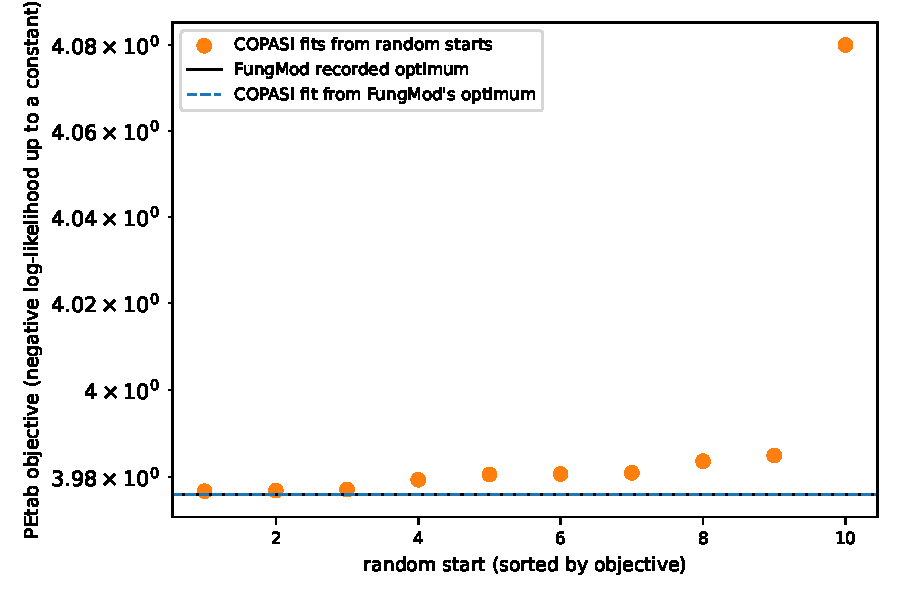
\includegraphics[width=0.7\textwidth]{figures/figure_4_cross_solver.pdf}
  \caption{Cross-solver check of the recorded optimum in COPASI. Objective
    of the exported three-condition PEtab problem at FungMod's recorded
    optimum, after COPASI's local fit from that point, and at the end of
    COPASI's fits from ten random starts (log axis). The recorded outcome is
    quoted in the manifest.}
  \label{fig:figure_4_cross_solver}
\end{figure}

\section{Relation to existing tools}

COPASI, SBML simulators and PEtab-based estimation frameworks are the
general infrastructure FungMod exports to, not alternatives to it; the
cross-solver study is the demonstration. Genome-scale metabolic
reconstructions address intracellular flux, not the extracellular
degradation dynamics, assay-defined activities and provenance bookkeeping
that FungMod models. Kinetic databases such as SABIO-RK \citep{wittig2012}
supply enzyme constants; FungMod imports them as sourced records (one
pH-response case is bound to a SABIO-RK entry) and keeps their conditions
attached.

\section{Limitations and claims not made}

\begin{itemize}
\item One organism, one substrate, one laboratory's data; no transfer to
  another strain, substrate or condition has been tested. A survey found no
  open raw-data deposit of a comparable submerged cellulose culture; figure
  digitisations with explicit digitisation uncertainty are the only
  candidates and need full-text review before use.
\item Every error model is an assumption because the deposit holds no
  replicates; the noise multiplier absorbs model misfit and measurement
  noise together.
\item Nutrient, oxygen and maintenance physiology are absent from the
  organism case; solid-substrate accessibility is a placeholder; there is no
  spatial mycelium.
\item The least-squares optimiser's finite-difference step was undeclared
  until the cross-solver check found it stopping 1.3 percent above the
  minimum; the public calibration API still uses scipy's default step and
  is not used by any recorded result in this paper.
\item The stage B chains did not reach the declared convergence rule within
  the plan's compute cap, the \texttt{M2} chain not even at the 36000 steps
  its amendment allowed; their verdicts are provisional.
\item Software verification (parity tests, reference simulators,
  cross-solver agreement) is not empirical validation, and this paper makes
  no predictive biological claim.
\end{itemize}

\section{Reproducibility and availability}

FungMod is MIT-licensed at \url{https://github.com/felixlaga/FungMod} with
documentation at \url{https://fungmod.readthedocs.io/}. Each study above has
a runner script, a frozen plan, a README and checksummed results. Every
table and figure in this paper is generated from those result files by one
command, \texttt{python scripts/reproduce\_paper.py tables}, which writes
the tables as \LaTeX{} fragments that this manuscript includes and the
figures as PDF files, together with a manifest naming each table's and
figure's source files, their SHA-256 digests and the numbers the text
quotes; the test suite fails if the committed tables, figures, the
manifests or the sources drift apart, or if the manuscript stops including
one of them. The same command has costlier tiers: \texttt{check} and
\texttt{verify} (seconds to a minute) recompute the digest chains, the
compiled-core objective at the recorded cross-solver optimum and the
stationarity of the recorded baseline fit without re-running any study;
\texttt{stage-a} re-runs the least-squares stage and the COPASI
reproduction (about two hours) and compares them with the recorded
summaries; \texttt{full} also re-runs the Bayesian study and the posterior
chains (a day of compute) and compares verdict-level fields, because seeded
chains can differ in individual samples across platforms. The runtime
dependency closure is pinned in \texttt{requirements-lock.txt}; continuous
integration builds the wheel, downloads that closure into a wheelhouse and
installs the wheel with network access disabled, then runs a virtual
experiment from outside the checkout. A tagged, archived release with a DOI
is \emph{pending}.

\section{AI assistance disclosure}

The code, studies and this draft were produced with substantial assistance
from an AI coding assistant (Claude Code, Anthropic) directed by the
author, under the repository's written rules on provenance, maturity
labels and forbidden shortcuts, with every scientific study run under a
plan frozen before its first fit. Human review of the biological mapping
and of this text is outstanding and is not claimed here.

\section*{Acknowledgements}

The Gelain et al.\ deposit (CC BY 4.0) made the organism case possible. The
COPASI, libSBML, PEtab and SciPy communities provided the tools the
cross-solver study depends on.

\bibliography{paper}

\end{document}
